% 本文件是示例论文的一部分
% 论文的主文件位于上级目录的 `main.tex`

\chapter{雨水资源GIS专题图详细设计与实现}

\section{功能设计}

\subsection{模块设计}
通过需求分析总体设计分析之后,将GIS专题图项目分为四个模块,主要为:大屏左面数据栏,右边数据栏,GIS专题图,头部导航栏四个模块,通过将数据展示栏和专题图还有导航栏分模块,可以使后期进行系统迭代更加方便,也符合模块化开发的标准和要求,主要模块分类如\ref{fig:module}所示:

\begin{figure}[!htb]%关于这些编译器的配置和使用,请参阅相关说明资料。
	\centering
	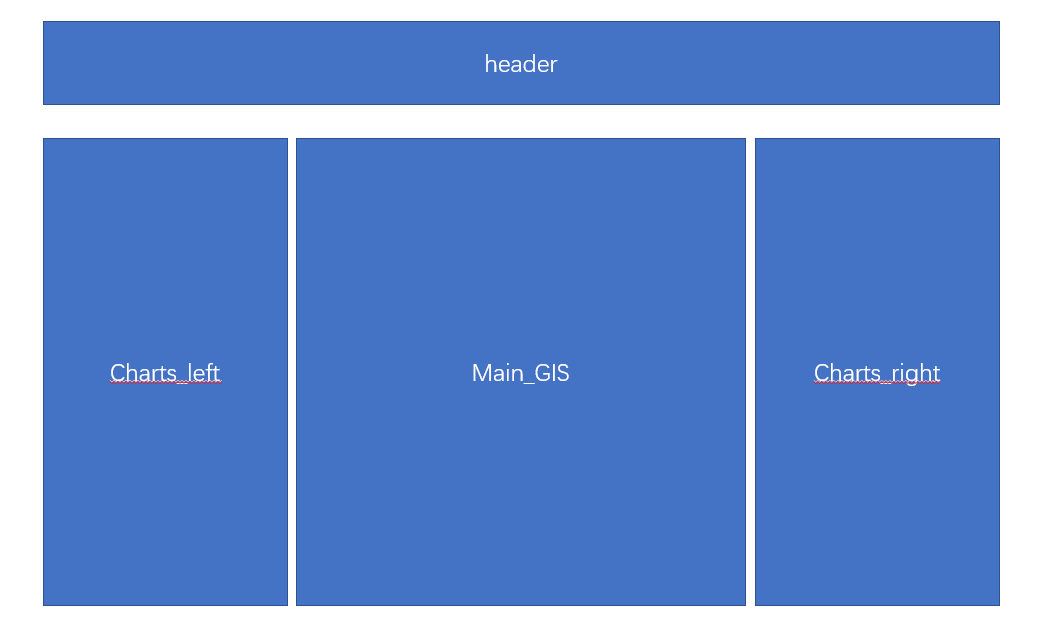
\includegraphics[width=0.60\textwidth]{figs/main.png}
	\caption{模块布局分类}
	\label{fig:module}
\end{figure}

\subsection{界面设计}


\section{地表水系设计}

\subsection{河流专题图设计}
\subsection{蓄水池专题图设计}
\subsection{水库专题图设计}
\section{地下水系设计}
\subsection{地下水分布专题图}
\subsection{土壤含量图}
\subsection{土壤类型图}
\section{气候图}
\subsection{光照专题图}
\subsection{降雨专题图}
\subsection{风速风向专题图}


%%% Local Variables: 
%%% mode: latex
%%% TeX-master: "../main.tex"
%%% End:
